\documentclass{standalone}
\usepackage{tikz}
\usetikzlibrary{patterns, positioning}
\usepackage[sfdefault]{ClearSans} %% option 'sfdefault' activates Clear Sans as the default text font
\usepackage[T1]{fontenc}

\begin{document}
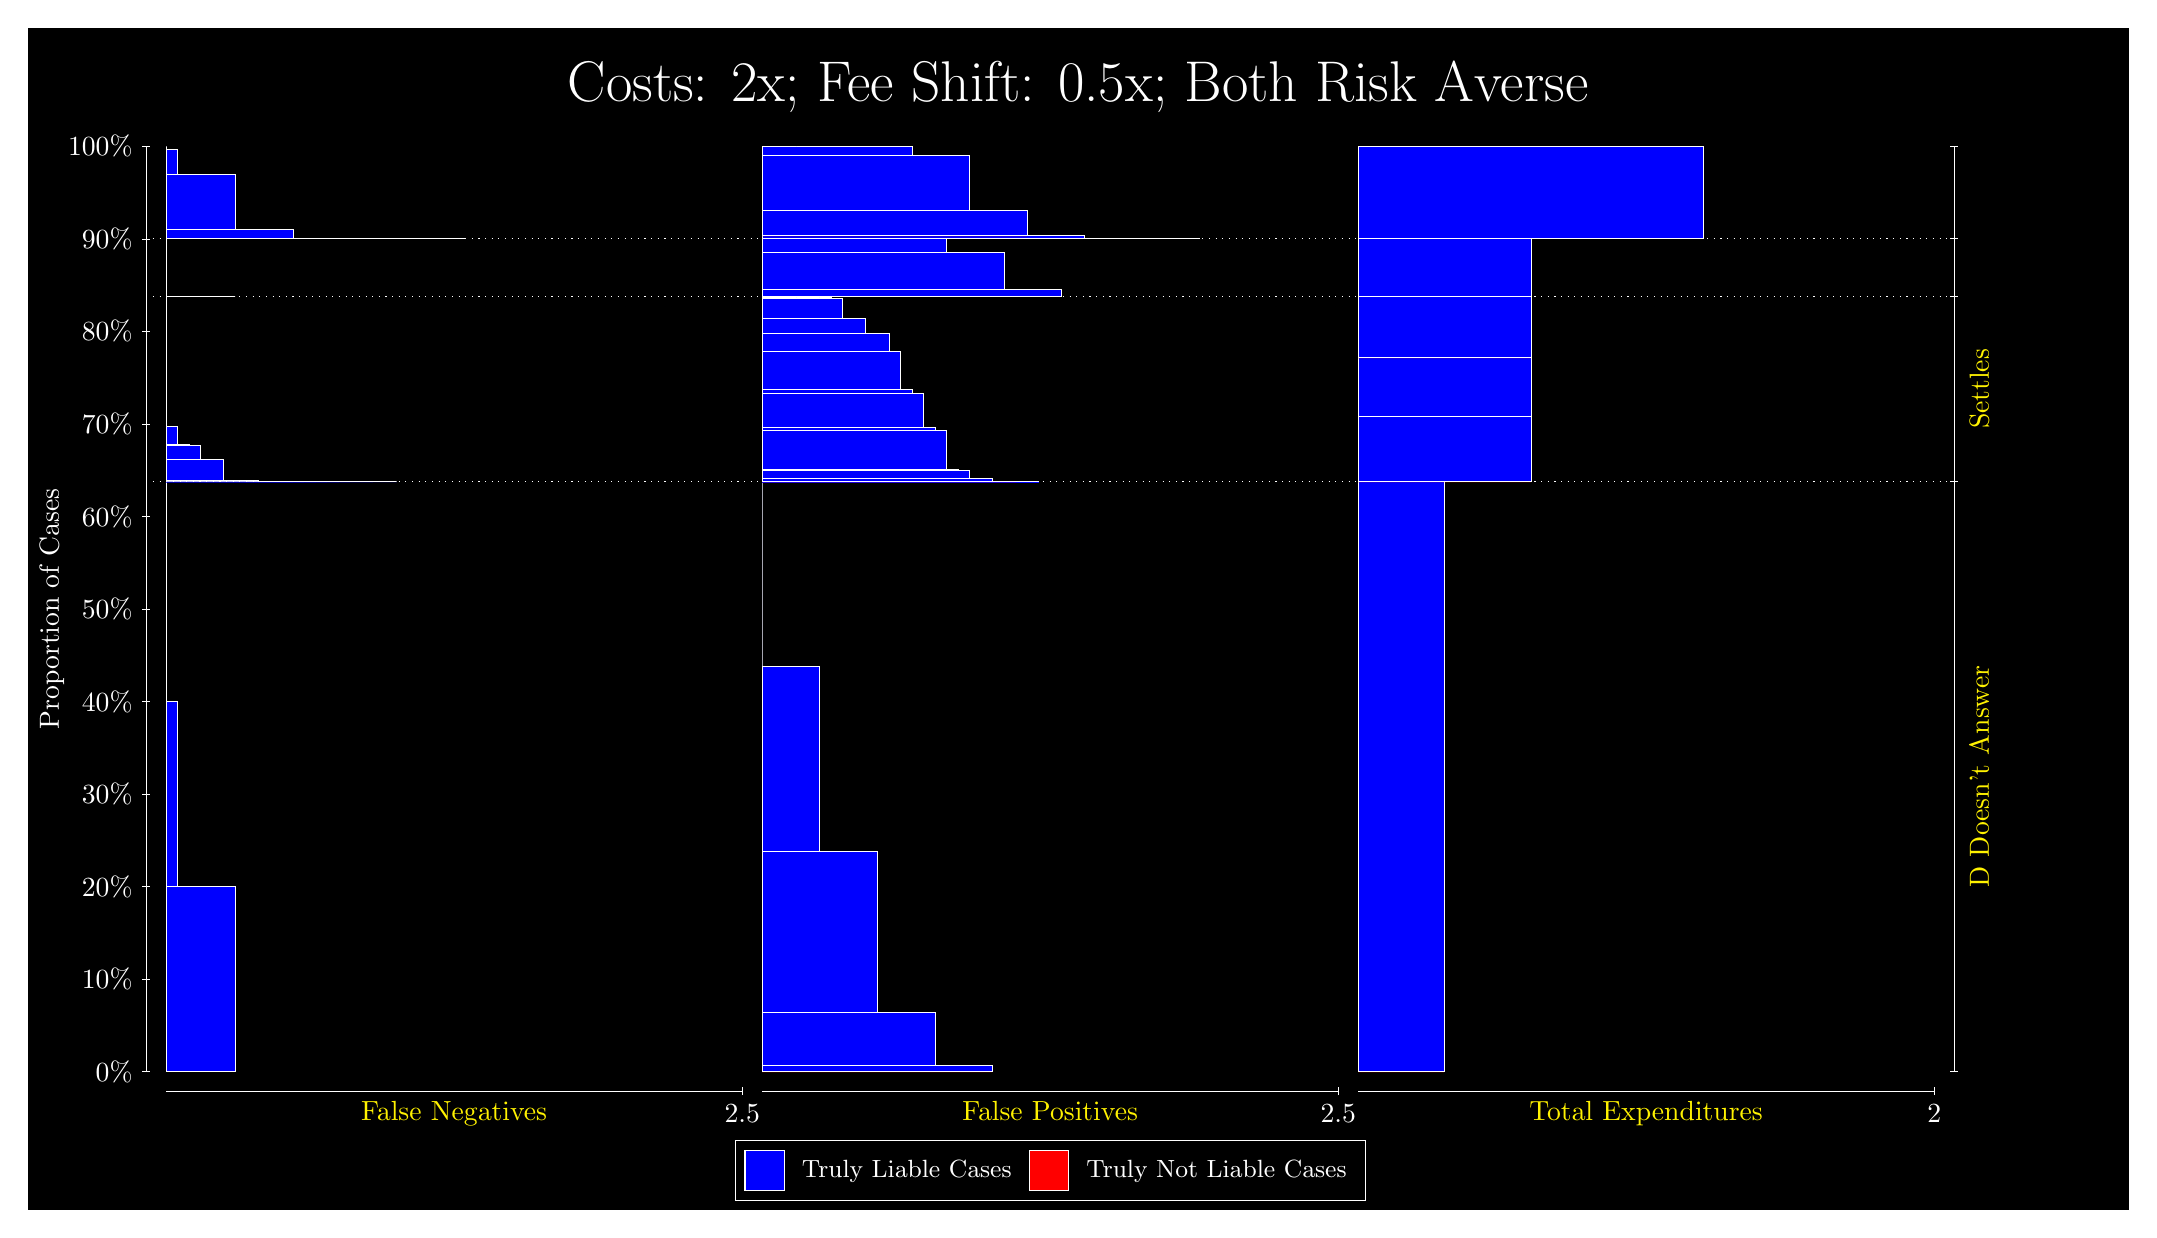
\begin{tikzpicture}
\draw[fill=black] (0,0) rectangle (26.667,15);
\draw[text=white] (0,13.5) rectangle (26.667,15) node[midway] {\huge Costs: 2x; Fee Shift: 0.5x; Both Risk Averse};
\draw[white, very thin] (1.5,1.75) -- (1.5,13.5);
\node[rotate=90, text=white, anchor=center] at (0.3, 7.625) {Proportion of Cases};
\draw[white, very thin] (1.45,1.75) -- (1.55,1.75);
\node[text=white, anchor=east] at (1.45, 1.75) {0\%};
\draw[white, very thin] (1.45,2.925) -- (1.55,2.925);
\node[text=white, anchor=east] at (1.45, 2.925) {10\%};
\draw[white, very thin] (1.45,4.1) -- (1.55,4.1);
\node[text=white, anchor=east] at (1.45, 4.1) {20\%};
\draw[white, very thin] (1.45,5.275) -- (1.55,5.275);
\node[text=white, anchor=east] at (1.45, 5.275) {30\%};
\draw[white, very thin] (1.45,6.45) -- (1.55,6.45);
\node[text=white, anchor=east] at (1.45, 6.45) {40\%};
\draw[white, very thin] (1.45,7.625) -- (1.55,7.625);
\node[text=white, anchor=east] at (1.45, 7.625) {50\%};
\draw[white, very thin] (1.45,8.8) -- (1.55,8.8);
\node[text=white, anchor=east] at (1.45, 8.8) {60\%};
\draw[white, very thin] (1.45,9.975) -- (1.55,9.975);
\node[text=white, anchor=east] at (1.45, 9.975) {70\%};
\draw[white, very thin] (1.45,11.15) -- (1.55,11.15);
\node[text=white, anchor=east] at (1.45, 11.15) {80\%};
\draw[white, very thin] (1.45,12.325) -- (1.55,12.325);
\node[text=white, anchor=east] at (1.45, 12.325) {90\%};
\draw[white, very thin] (1.45,13.5) -- (1.55,13.5);
\node[text=white, anchor=east] at (1.45, 13.5) {100\%};

\draw[white, very thin] (24.457,1.75) -- (24.457,13.5);
\draw[white, very thin] (24.407,1.75) -- (24.507,1.75);
\node[anchor=west] at (24.407, 1.75) {};
\draw[white, very thin] (24.407,9.2415) -- (24.507,9.2415);
\node[anchor=west] at (24.407, 9.2415) {};
\draw[white, very thin] (24.407,11.597) -- (24.507,11.597);
\node[anchor=west] at (24.407, 11.597) {};
\draw[white, very thin] (24.407,12.332) -- (24.507,12.332);
\node[anchor=west] at (24.407, 12.332) {};
\draw[white, very thin] (24.407,13.5) -- (24.507,13.5);
\node[anchor=west] at (24.407, 13.5) {};

\draw[white, very thin, fill=blue] (1.75,1.75) rectangle (2.6283,4.0999);
\draw[white, very thin, fill=blue] (1.75,4.0999) rectangle (1.8964,6.4473);
\draw[white, very thin, fill=red] (1.75,6.4473) rectangle (1.75,6.4473);
\draw[white, very thin, fill=blue] (1.75,6.4473) rectangle (1.75,9.2415);
\draw[white, very thin, fill=blue] (1.75,9.2415) rectangle (4.6775,9.2415);
\draw[white, very thin, fill=blue] (1.75,9.2415) rectangle (4.3848,9.2415);
\draw[white, very thin, fill=blue] (1.75,9.2415) rectangle (4.092,9.2415);
\draw[white, very thin, fill=blue] (1.75,9.2415) rectangle (3.9457,9.2415);
\draw[white, very thin, fill=blue] (1.75,9.2415) rectangle (3.7993,9.2415);
\draw[white, very thin, fill=blue] (1.75,9.2415) rectangle (3.6529,9.2415);
\draw[white, very thin, fill=blue] (1.75,9.2415) rectangle (3.5065,9.2415);
\draw[white, very thin, fill=blue] (1.75,9.2415) rectangle (3.3602,9.2415);
\draw[white, very thin, fill=blue] (1.75,9.2415) rectangle (3.2138,9.2501);
\draw[white, very thin, fill=blue] (1.75,9.2501) rectangle (3.0674,9.2501);
\draw[white, very thin, fill=blue] (1.75,9.2501) rectangle (2.921,9.2556);
\draw[white, very thin, fill=blue] (1.75,9.2556) rectangle (2.921,9.2556);
\draw[white, very thin, fill=blue] (1.75,9.2556) rectangle (2.7746,9.2556);
\draw[white, very thin, fill=blue] (1.75,9.2556) rectangle (2.6283,9.2627);
\draw[white, very thin, fill=blue] (1.75,9.2627) rectangle (2.4819,9.5236);
\draw[white, very thin, fill=blue] (1.75,9.5236) rectangle (2.3355,9.5254);
\draw[white, very thin, fill=blue] (1.75,9.5254) rectangle (2.1891,9.7082);
\draw[white, very thin, fill=blue] (1.75,9.7082) rectangle (2.1891,9.7083);
\draw[white, very thin, fill=blue] (1.75,9.7083) rectangle (2.0428,9.7137);
\draw[white, very thin, fill=blue] (1.75,9.7137) rectangle (1.8964,9.9436);
\draw[white, very thin, fill=red] (1.75,9.9436) rectangle (1.75,9.9436);
\draw[white, very thin, fill=blue] (1.75,9.9436) rectangle (1.75,11.597);
\draw[white, very thin, fill=blue] (1.75,11.597) rectangle (2.6283,11.597);
\draw[white, very thin, fill=blue] (1.75,11.597) rectangle (1.8964,11.599);
\draw[white, very thin, fill=red] (1.75,11.599) rectangle (1.75,11.599);
\draw[white, very thin, fill=blue] (1.75,11.599) rectangle (1.75,12.332);
\draw[white, very thin, fill=blue] (1.75,12.332) rectangle (5.5558,12.332);
\draw[white, very thin, fill=blue] (1.75,12.332) rectangle (4.8239,12.332);
\draw[white, very thin, fill=blue] (1.75,12.332) rectangle (4.092,12.334);
\draw[white, very thin, fill=blue] (1.75,12.334) rectangle (3.3602,12.452);
\draw[white, very thin, fill=blue] (1.75,12.452) rectangle (2.6283,12.452);
\draw[white, very thin, fill=blue] (1.75,12.452) rectangle (2.6283,13.146);
\draw[white, very thin, fill=blue] (1.75,13.146) rectangle (1.8964,13.146);
\draw[white, very thin, fill=blue] (1.75,13.146) rectangle (1.8964,13.468);
\draw[white, very thin, fill=red] (1.75,13.468) rectangle (1.75,13.468);
\draw[white, very thin, fill=blue] (1.75,13.468) rectangle (1.75,13.5);
\draw[white, very thin, fill=red] (9.3189,1.75) rectangle (12.246,1.75);
\draw[white, very thin, fill=blue] (9.3189,1.75) rectangle (12.246,1.8338);
\draw[white, very thin, fill=blue] (9.3189,1.8338) rectangle (11.515,2.4997);
\draw[white, very thin, fill=blue] (9.3189,2.4997) rectangle (10.783,4.5442);
\draw[white, very thin, fill=blue] (9.3189,4.5442) rectangle (10.051,6.8916);
\draw[white, very thin, fill=blue] (9.3189,6.8916) rectangle (9.3189,9.2415);
\draw[white, very thin, fill=red] (9.3189,9.2415) rectangle (12.832,9.2415);
\draw[white, very thin, fill=blue] (9.3189,9.2415) rectangle (12.832,9.2418);
\draw[white, very thin, fill=red] (9.3189,9.2418) rectangle (12.539,9.2418);
\draw[white, very thin, fill=blue] (9.3189,9.2418) rectangle (12.539,9.244);
\draw[white, very thin, fill=red] (9.3189,9.244) rectangle (12.246,9.244);
\draw[white, very thin, fill=blue] (9.3189,9.244) rectangle (12.246,9.2791);
\draw[white, very thin, fill=blue] (9.3189,9.2791) rectangle (12.1,9.2891);
\draw[white, very thin, fill=red] (9.3189,9.2891) rectangle (11.954,9.2891);
\draw[white, very thin, fill=blue] (9.3189,9.2891) rectangle (11.954,9.3894);
\draw[white, very thin, fill=blue] (9.3189,9.3894) rectangle (11.807,9.4034);
\draw[white, very thin, fill=red] (9.3189,9.4034) rectangle (11.661,9.4034);
\draw[white, very thin, fill=blue] (9.3189,9.4034) rectangle (11.661,9.8924);
\draw[white, very thin, fill=blue] (9.3189,9.8924) rectangle (11.515,9.9367);
\draw[white, very thin, fill=red] (9.3189,9.9367) rectangle (11.368,9.9367);
\draw[white, very thin, fill=blue] (9.3189,9.9367) rectangle (11.368,10.359);
\draw[white, very thin, fill=blue] (9.3189,10.359) rectangle (11.222,10.415);
\draw[white, very thin, fill=blue] (9.3189,10.415) rectangle (11.075,10.419);
\draw[white, very thin, fill=red] (9.3189,10.419) rectangle (11.075,10.419);
\draw[white, very thin, fill=blue] (9.3189,10.419) rectangle (11.075,10.895);
\draw[white, very thin, fill=blue] (9.3189,10.895) rectangle (10.929,11.125);
\draw[white, very thin, fill=blue] (9.3189,11.125) rectangle (10.783,11.13);
\draw[white, very thin, fill=blue] (9.3189,11.13) rectangle (10.636,11.313);
\draw[white, very thin, fill=blue] (9.3189,11.313) rectangle (10.49,11.315);
\draw[white, very thin, fill=blue] (9.3189,11.315) rectangle (10.344,11.315);
\draw[white, very thin, fill=blue] (9.3189,11.315) rectangle (10.344,11.576);
\draw[white, very thin, fill=blue] (9.3189,11.576) rectangle (10.197,11.583);
\draw[white, very thin, fill=blue] (9.3189,11.583) rectangle (10.051,11.583);
\draw[white, very thin, fill=blue] (9.3189,11.583) rectangle (9.9044,11.588);
\draw[white, very thin, fill=blue] (9.3189,11.588) rectangle (9.758,11.588);
\draw[white, very thin, fill=blue] (9.3189,11.588) rectangle (9.6116,11.588);
\draw[white, very thin, fill=blue] (9.3189,11.588) rectangle (9.6116,11.597);
\draw[white, very thin, fill=blue] (9.3189,11.597) rectangle (9.4652,11.597);
\draw[white, very thin, fill=blue] (9.3189,11.597) rectangle (9.3189,11.597);
\draw[white, very thin, fill=red] (9.3189,11.597) rectangle (13.125,11.597);
\draw[white, very thin, fill=blue] (9.3189,11.597) rectangle (13.125,11.684);
\draw[white, very thin, fill=blue] (9.3189,11.684) rectangle (12.393,12.149);
\draw[white, very thin, fill=blue] (9.3189,12.149) rectangle (11.661,12.331);
\draw[white, very thin, fill=blue] (9.3189,12.331) rectangle (10.929,12.332);
\draw[white, very thin, fill=blue] (9.3189,12.332) rectangle (10.197,12.332);
\draw[white, very thin, fill=red] (9.3189,12.332) rectangle (14.881,12.332);
\draw[white, very thin, fill=blue] (9.3189,12.332) rectangle (14.881,12.332);
\draw[white, very thin, fill=red] (9.3189,12.332) rectangle (14.149,12.332);
\draw[white, very thin, fill=blue] (9.3189,12.332) rectangle (14.149,12.333);
\draw[white, very thin, fill=red] (9.3189,12.333) rectangle (13.417,12.333);
\draw[white, very thin, fill=blue] (9.3189,12.333) rectangle (13.417,12.364);
\draw[white, very thin, fill=red] (9.3189,12.364) rectangle (12.686,12.364);
\draw[white, very thin, fill=blue] (9.3189,12.364) rectangle (12.686,12.686);
\draw[white, very thin, fill=red] (9.3189,12.686) rectangle (11.954,12.686);
\draw[white, very thin, fill=blue] (9.3189,12.686) rectangle (11.954,13.38);
\draw[white, very thin, fill=blue] (9.3189,13.38) rectangle (11.222,13.498);
\draw[white, very thin, fill=blue] (9.3189,13.498) rectangle (10.49,13.5);
\draw[white, very thin, fill=blue] (9.3189,13.5) rectangle (9.758,13.5);
\draw[white, very thin, fill=blue] (9.3189,13.5) rectangle (9.3189,13.5);
\draw[white, very thin, fill=red] (16.888,1.75) rectangle (17.986,1.75);
\draw[white, very thin, fill=blue] (16.888,1.75) rectangle (17.986,9.2415);
\draw[white, very thin, fill=red] (16.888,9.2415) rectangle (19.083,9.2415);
\draw[white, very thin, fill=blue] (16.888,9.2415) rectangle (19.083,10.073);
\draw[white, very thin, fill=red] (16.888,10.073) rectangle (19.083,10.073);
\draw[white, very thin, fill=blue] (16.888,10.073) rectangle (19.083,10.818);
\draw[white, very thin, fill=red] (16.888,10.818) rectangle (19.083,10.818);
\draw[white, very thin, fill=blue] (16.888,10.818) rectangle (19.083,11.597);
\draw[white, very thin, fill=red] (16.888,11.597) rectangle (19.083,11.597);
\draw[white, very thin, fill=blue] (16.888,11.597) rectangle (19.083,12.332);
\draw[white, very thin, fill=red] (16.888,12.332) rectangle (21.279,12.332);
\draw[white, very thin, fill=blue] (16.888,12.332) rectangle (21.279,13.5);
\draw[white, dotted] (1.5,9.2415) -- (24.457,9.2415);
\draw[white, dotted] (1.5,11.597) -- (24.457,11.597);
\draw[white, dotted] (1.5,12.332) -- (24.457,12.332);
\draw[white, very thin] (1.75,1.5) -- (9.0689,1.5);
\node[text=yellow, anchor=north] at (5.4094, 1.5) {False Negatives};
\draw[white, very thin] (9.0689,1.45) -- (9.0689,1.55);
\node[text=white, anchor=north] at (9.0689, 1.45) {2.5};

\draw[white, very thin] (9.3189,1.5) -- (16.638,1.5);
\node[text=yellow, anchor=north] at (12.978, 1.5) {False Positives};
\draw[white, very thin] (16.638,1.45) -- (16.638,1.55);
\node[text=white, anchor=north] at (16.638, 1.45) {2.5};

\draw[white, very thin] (16.888,1.5) -- (24.207,1.5);
\node[text=yellow, anchor=north] at (20.547, 1.5) {Total Expenditures};
\draw[white, very thin] (24.207,1.45) -- (24.207,1.55);
\node[text=white, anchor=north] at (24.207, 1.45) {2};

\node[text=yellow, centered, rotate=90] at (24.777, 5.4958) {D Doesn't Answer};
\node[text=yellow, centered, rotate=90] at (24.777, 10.419) {Settles};



\draw (12.978300999999998,1.5) node[draw=none] (baseCoordinate) {};
\begin{scope}[align=center]
        \matrix[scale=0.5, draw=white, below=0.5cm of baseCoordinate, nodes={draw}, column sep=0.1cm]{
            \node[rectangle, draw, minimum width=0.5cm, minimum height=0.5cm, fill=blue] {}; &
            \node[draw=none, font=\small, text=white] (B) {Truly Liable Cases}; &
            \node[rectangle, draw, minimum width=0.5cm, minimum height=0.5cm, fill=red] {}; &
            \node[draw=none, font=\small, text=white] (B) {Truly Not Liable Cases}; \\
            };
\end{scope}

\end{tikzpicture}
\end{document}